\chapter{Muutused äris}

\section{Struktuursed ja mittestruktuursed muutused}
Analüüsides ärimuutust on oluline mõista, millistes organisatsiooni kihtides (Vt. joonis \ref{fig:stack} leheküljel \pageref{fig:stack}) on tegemist struktuurse ja millistes mittestruktuurse muutusega. Struktuurne on muutus, mis muudab kihi arhitektuuri samas kui mittestruktuurne jätab selle muutmata. Küsimus on oluline, sest arhitektuuri muutmine on, vastupidiselt olemasoleva arhitektuuri raames toimetamisega, reeglina kallis.

Võtkem näiteks ettevõtte, kes müüb oma teenuseid e-poe kaudu. Tehakse otsus, et veebilehele tuleb lisada võimalus klienditoega sõnumivahetusse asuda. Sellist funktsionaalsust pakkuvaid tarkvarapakette on palju ning nende integreerimine olemasolevasse tehnilisse lahendusse reeglina ei ole probleem. Tegu ei ole struktuurse muutusega, olemasolev arhitektuur jääb paika. Samas on organisatsioonis 24/7 toimiva klienditoe funktsiooni arendamine äriprotsesside ja organisatsiooni struktuuri mõttes üsna keeruline ettevõtmine. Tuleb palgata ööpäevaringse valve mehitamiseks piisav hulk inimesi ning nende juht, organiseerida juurdepääs kontoripinnale, tõeäoliselt tegeleda tööseadusandlusest tulenevate piirangutega jne. jne. Selgesti on tegemist arhitektuurse muutusega. 

Tüüpilisemad on vastupidised näited kus organisatsiooni vaatest triviaalne muutus võib osutuda tehnilises mõttes uut arhitektuuri nõudvaks. Otsused tulevad just organisatsiooni vaadet omavatelt inimestelt kes lihtsa muutuse palju suurema tõenäosusega ette võtavad kui keerulise. 

Et arhitektuuri mõiste ei ole hästi defineeritud ei ole ka struktuurne ja mittestruktuurne muutus selgepiirilised mõisted. Selge on siiski, et erinevad muudatused vajavad erineva hulga olemasoleva välja vahetamist ning just see on küsimuse iva.

\section{Keerukus ja keerulisus}
\TODO Kirjuta slaidide alusel lahti. Keerulisuse juures võimude pilt

\section{Kuidas mõõta infosüsteemi keerukust?}
\label{sec:complexity}
\cite{mitchell2009complexity} toob välja rea keerukuse mõõtmise viise. \citeauthor{crawley2015systems}\cite{crawley2015systems} toob välja mitmeid konkreetseid valemeid keerukuse arvutamiseks. Kuna variatsioone teema ümber on arvukalt ning nende erivused ei ole siinkohal määrava tähtsusega, kasutame keerukuse hindamisel järgmist valemit. 

\begin{equation}
	C = \sqrt[3]{N_e + N_et + N_s + N_st}
	\label{eq:complexity}
\end{equation}

\begin{itemize}
	\item $N_e$ on elementide hulk süsteemis
	\item $N_{et}$ on elementide tüüpide hulk süsteemis
	\item $N_s$ on elementidevaheliste seoste hulk süsteemis
	\item $N_{st}$ on elementidevaheliste seoste hulk süsteemis
\end{itemize}

Valemi sisu on lihtne: süsteemi keerukus määratletakse kui lineaarsest aeglasemalt kasvavat summat elementidest, seostest ja nende liikidest. 

Vaatleme selle valemi rakendamist lihta ülesande näitel. Olgu meil ülesanne liiklust läbi kahest komponendi - turvaserverist ja infosüsteemist - koosnevas süsteemis. Turvaserver saab väliskeskkonnast päringu ja edastab selle infosüsteemile töötlemiseks. Süsteemi põhimõtteline paigaldusskeem on toodud jooonisel \ref{fig:complexity:pure}.

\begin{figure}[htp]
	\begin{center}
		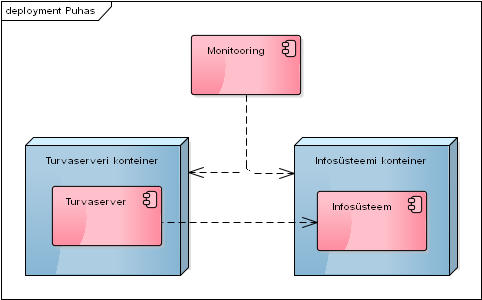
\includegraphics[width=.6\textwidth]{puhas.png}
		\caption{Jälgitava süsteemi põhimõtteline paigaldusskeem}
		\label{fig:complexity:pure}
	\end{center}
\end{figure}

Süvenemata realisatsiooni detailidesse võib öelda, et leidub kaks põhimõttelist viisi liikluse jälgimiseks. Esimene koosneb eraldi paigaldatavast vahendajast turvaserveri ja infosüsteemi vahel. Vahendaja pakub sama liidest, mis infosüsteem ja edastab ühele poole päringuid ja teisele vastuseid. Teine koosneb turvaserveri ümber mässitavast lahendusest, mis jälgib turvaserverisse sisenevat liiklust ning edastab selle turvaserverile. Peamine vahe alternatiivide vahel on eraldi (virtuaal)serveri vajadus esimesel juhul. Alternatiivid on toodud joonisel \ref{fig:complexity:added}.


\begin{figure}[ht]
		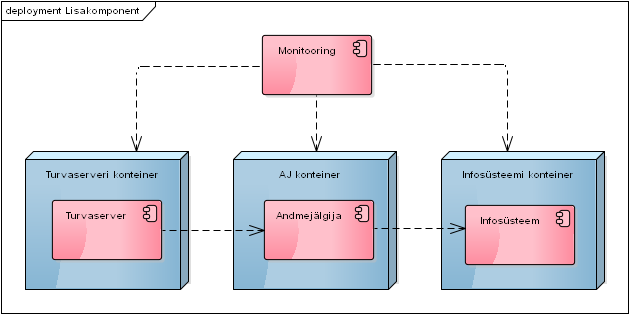
\includegraphics[width=8cm]{lisakomponent.png}
		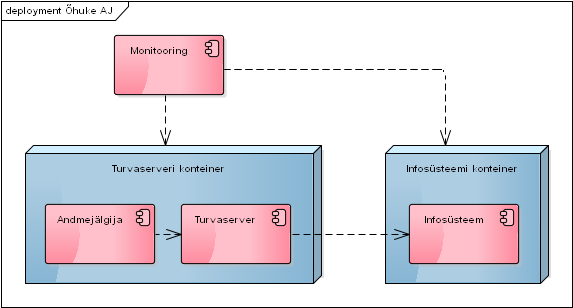
\includegraphics[width=8cm]{ohuke.png}
		\caption{Kaks alternatiivi andmete jälgimiseks}
		\label{fig:complexity:added}
\end{figure}

Esmapilgul ei ole alternativiide erinevus keerukuse mõttes ilmselged. Loendades valemi \ref{eq:complexity} muutujate väärutsi ilma andmejälgijata leiame, et süsteemis on viis elementi (kaks konteinerit ja kolm tarkvarakomponenti), neli liidest (turvaserveri sisenev, infosüsteemi sisenev ning monitooringuliidesed) ning et nii elemente kui liideseid on kahte tüüpi. Eraldi paigaldatava andmejälgija puhul saame vastavalt väärtused 7, 7, 2 ja 2. Õhukese lahenduse puhul väheneb küll elementide arv kuid lisandub uus liidese tüüp protsesside vaheliseks suhtluseks konteineri sees. Tulemused võtab kokku tabel \ref{tab:complexity}. 

Näeme, et andmejälgija iseenesest lisab süsteemi oluliselt keerukust. Samas on alternatiivne, turvaserveriga kokku paigaldatav, lahendus õige pisut väiksema keerukusega. Loomulikult on tegu lihtsustatud näitega kuid tegu on reaalse viisiga kvantifitseerida arhitektuursete lahenduste erinevusi. Tasub ka tähele panna, et süsteemi piiride määratlemisel on oluline mõju: kui lugeda süsteemi keerukuse hulka ka turvaserverisse sisenev liides, suureneb alternatiivide poolt jagatud liideste hulk ning seega väheneb suhteline erinevus. 

\begin{table}
	\begin{center}
		\begin{tabular}{p{3.6 cm}rrr}
		\toprule
& Puhas & Eraldi AJ & Õhuke AJ \\
		\midrule
Elemente ($N_e$) &	5 &	7 &	6\\
Liideseid  ($N_s$)	& 4 &	7 &	6\\
Elementide liike  ($N_{et}$)&	2	&2	&2\\
Liideste liike  ($N_{st}$)&	2 &	2 &	3\\
		\midrule
Keerukus &	2.35 &	2.62	 &2.57\\
		\bottomrule
		\end{tabular}
		\caption{Kokkuvõte alternatiivide keerukusest}
		\label{tab:complexity}

	\end{center}
\end{table}

\section{Demokraatlikust innovatsioonist}
Innovatsioonist on lihtne mõelda kui millestki pool-müstilisest. Selle ümber tiirleb hulk särava jutuga tegelasi, tehakse teadust ning sellele \enquote{pannakse rõhku}. Ometi on inimene aastatuhandeid suurema kärata innovatsiooniga tegelenud. Erinevalt moodsast ühiskonnast, paar tuhat aastat tagasi ilmselt ei leidunud palju innovatsiooni oma ametiks pidavaid inimesi. Ometi tehnoloogia liikus ning inimkond arenes. Kuidas?

Nutikad inimesed lihtsalt lahendasid käepäraste vahenditega endi ees seisvaid probleeme. Pähkli katki toksimiseks sobis terava servaga kivi tömbist paremini ja ühel hetkel taipas keegi, et kivi saab ise teritada. Selgub\cite{hippel}, et sarnased mehhanismid toimivad ka täna: mitmesugused leiutised Apache veebiserveri turvavõimalustest kunstliku vereringe masinaga on sündinud kellegi vajadusest oma pakiline probleem lahendada. Ka Skype sündis inimeste praktilisest vajadusest odavalt kaugekõnesid teha. 

Ometi ei ole me kõik maailmakuulsad leidurid. Kõik meie probleemid lihtsalt ei ole piisavalt universaalsed, et laialt levida. Demokraatliku innovatsiooni puhul ongi oluline hetk, kus leiutis muutub lahendusest leiutaja(te) probleemile lahenduseks kellegi teise probleemile. Sel hetkel muutub fookus ja selgub probleemi tegelik levik klientide hulgas. 

Tarkvarainsenerid on loomult keskmisest leidlikumad, nende seas on levinud häkkeri-mentaliteet ning seetõttu on nad varmad oma probleeme ise lahendama. Erinevalt füüsilisest maailmast on tarkvaralised lahendused ka lihtsasti levitatavad. Seetõttu on maailm täis kõikvõimalikke vabaralisi platvorme, milledest mitte kõik ei ole laialt kasutusel ega elujõulised. 

Seega võib IT olla kergesti ärilise muutuse algatajaks. Ühest küljest on küsimus usalduses: kas ja mil määral usub organisatsiooni juhtkond IT võimesse õigesti hinnata probleemi universaalsust\sidenote{Skypel oli olemas Twitteriga väga sarnane funktsionaalsus vähemalt aasta enne Twitteri käivitamist. Seda ei pakendatud kunagi tooteks, sest organisatsiooni fookus oli mujal}. Teisalt on vahel tegemist leiutistega, \enquote{millede aeg ei ole veel käes}\sidenote{\quote{\enquote{Nothing is stronger than an idea whose time has come}} Victor Hugo}. Tihti võib millegi laiemaks levikuks olla tarvis soodsat majanduslikku kliimat, mõnd võtmetehnoloogiat või muud sellist. Virtuaalreaalsus on mingil kujul olemas olnud alates eelmise sajandi kolmekümnendatest kuid alles 2016. aastal jõuavad turule esimesed tavakasutajale mõistliku hinnaga mõistlikku kogemust pakkuvad seadmed. 

Kolmanda külje alt võib küsimus olla ka ärimudelis või konkurentsisituatsioonis. 2016. aastal teatas Facebook oma \enquote{botipoe} avamisest\sidenote{\url{http://techcrunch.com/2016/03/17/facebooks-messenger-in-a-bot-store}} ning Skype teatas peatest võimalusest virtuaalse assistendiga sõnumeid vahetada\sidenote{\url{http://www.theverge.com/2016/3/30/11332424/skype-cortana-bot-interactions-messaging}}. Ometi on sõnumite kaudu käsklustele reageerivad robotid olemas olnud alates seitsmekümnendatest ning kas Skypel oli vastav idee juba ammu kasutusel\sidenote{Vähemalt kümnend enne viidatud uudiseid toimis Skypes niinimetatud \enquote{buildbot}. See oli tükk tarkvara, kes suutis sõnumeid vastu võtta, oli suuteline neid interpreteerima ning tegeles Skype kliendi eri versioonide kompileerimise ja pakendamisega}. Piisas vaid ühel osapoolel astuda samme idee tootestamiseks, kui teised olid oma strateegilise positsiooni säilitamiseks sama tegema.

Ehk, ITst tuleneva innovatsiooni kasutuselevõtu teel on hulgaliselt takistusi. Mistõttu nende ideedega inimesed võivad kergesti frustreeruda. Nende ideede geniaalsust ju ei mõisteta! Selle frustratsiooni juhtimine ja konstruktiivseks kanaliseerimine on üks IT-juhi raskematest ülesannetest. On ju ideede kasutuselevõtu vastu vahel ratsionaalseid argumente ning ka inimeste oma iduettevõtte loomisele suunamine ei ole ju tööandjale kasulik. Nagu pole kasulik ka andekas inimene, kes peab kolleege võimetuks oma ideid mõistma. 

\section{Küsimused aruteluks}
\subsection{Kas IT saab algatada organisatsiooni äri muutuse? Kui jah, siis kuidas?}
Üheks viisiks küsimuse üle arutleda on tagasipöördumine süsteemi kolme aspekti - vormi, funktsiooni ja kontseptsiooni - juurde. Nagu räägitud, annab kontseptsioon aluse vajaliku funktsionaalsuse realiseerimiseks konkreetse vormi abil. Kuna sama funktsiooni võib täita mitu vormi ja vastupidi, vajame kontseptsiooni, mis kahe hulga vahele seose tekitaks. 

Siit järeldub, et ka konkreetset funktsiooni realiseeriv vorm võib täita erinevaid funktsioone. Nuga loodi algul ilmselt tööriistana kuid võeti kiiresti kasutusele relvana. Ja siit tulebki üks IT võimalustest äri muuta: kui olemasolev vorm suudaks lisaks planeeritule veel midagi, saaks tolle miski äriks keerata investeerimata sentigi vormi muutusse ning kohandades vaid kontseptsiooni. 

Heaks näiteks on e-residentsus\index{E-residentsus}. Kuna kogu ID-kaarti ja e-teenuseid toetav taristu on igal juhul olemas (ning koormuse mõttes väga kaugel skaleeruvusprobleemidest) ei nõua paljut nonde kaartide välja andmine kellele iganes. Muutes riigi kodaniku kontseptsiooni\index{Kontseptsioon}, saab sama vormi abil realiseerida oluliselt laiemat funktsiooni. 

Siit ei tulene, et kogu loodav vorm peaks olema nii laia kasutusvõimalusega, kui võimalik. Tihti nii mõeldakse ja tulemuseks on kasutud platvormid, üliabstraktsed \enquote{konfigureeritavad} süsteemid ja, laias plaanis, üleinvesteerimine ITsse. Vorm peab olema optimaalne olemasoleva kontseptsiooni piirides. Järelikult on IT ülesanne lisaks potentsiaalsete uute funktsioonide tuvastamisele ka sellise süstemi kontseptsiooni arendamine, mis viiks võimalikult \enquote{lahtiste} ja mitmekülgsete vormideni. Kuigi kontseptsioon tuleneb suurel määral organisatsiooni kultuurist, on teda konkreetsetel juhtudel siiski võimalik mõjutada peegeldades kliendile tagasi sisendist mõnevõrra üldisemaid kontseptsioone. 

Ka siin tuleb loomulikult silmas pidada arenduse-halduse-äri kolmikut ning anda endale aru, millal soov kontseptsiooni arendada on tegelikult maskeeritud soov endale monumenti ehitada.

\subsection{Mida teha, kui ees olev muutus viib organisatsiooni teisele poole oma võimete piiri?}
Keerukusel\index{Keerukus} on komme eksponentsiaalselt kasvada (vt. joonis \ref{fig:complexity:growth}) ja nii võib kergesti juhtuda, et seni edukalt astutud sammudest järgmine viib meid teisele poole meie võimete piiri. Tulemuseks on meie võimetus süsteemi (nii tehnilist kui organisatsioonilist) hoomata ning seega ka juhtida. 

\begin{marginfigure}
		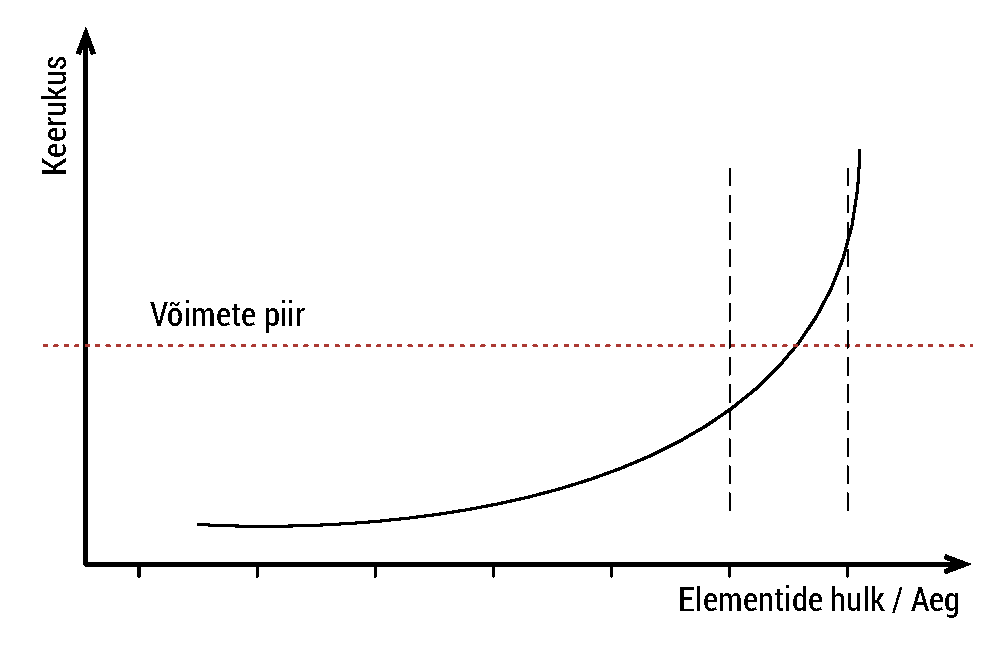
\includegraphics[width=\linewidth]{keerukus.pdf}
		\caption{Keerukuse eksponentsiaalne kasv teisele poole võimete piiri}
		\label{fig:complexity:growth}
\end{marginfigure}


Püstitatud küsimus on oluline, sest, eriti avalikus sektoris, ei ole muutus äris tihti ei välditav ega mõjutatav. Kui demokraatlik protsess on mingi tulemuse andnud, tuleb sellega leppida. Seda ka siis, kui organisatsioon seda välja ei kannata. Ideaalis muidugi võetakse organisatsiooni võimekust muudatust algatades arvesse kuid ei avalikus- ega erasektoris seda reeglina ei juhtu. Põhjuseks enamasti, et ei suudeta eristada objektiivset subjektiivsest. Ehk, kas läks vussi seepärast, et elluviijad osutusid saamatuks või seepärast, et ülesanne oligi antud kontekstis lahendamatu? Esimene variant on kindlasti käepärasem ning tavaliselt on otsustajate puhul mängus olulised positiivset mõtlemist soodustavad tegurid. 

Kuidas ka ei oleks, oleme me vastakuti muutusega, mis ei saa hästi lõppeda. Valgus tunneli lõpus on rong. Mida siis teha? 

Keerukuse juhtimiseks on meil juba mudelist tulenevalt kolm põhimõttelist strateegiat:
	\begin{description}
		\item[Google mudel:] \index{Google}Joone tõusu vähendamine. Me mõtleme välja, kuidas iga järgmine samm meie keerukust järjest vähem suurendaks. Kui google lisab oma farmi järgmise serveri, ei muuda see nende jaoks suurt midagi\sidenote{Google tarvitab oma serverite jaoks suurusjärgus 260 gigavatti võimsust (\url{https://www.technologyreview.com/s/425384/what-it-takes-to-power-google/}), ka massiivse gigavatise serveriruumi käivitamine ei muuda suurt midagi}. Ka järgmise teenuse või isegi äriliini käivitamine on tehtud suhteliselt lihtsaks. Google kogu äriedu tugineb nende võimel teha asju väga suurtes mastaapides, hoida oma keerukuskõver lamedana.
		\item[Morgani mudel:]\index{Morgan Motor Company} Peatumine horisontaalteljel. Briti autotootja Morgan on teinud põhimõttelise otsuse mitte areneda. Kasvu, keerukama tehnoloogia ja seega suurema tehnilise ja organisatsioonilise keerukuse asemel on jäädud piiratud mahtude ja käsitsi puust raamile loodavate autode juurde. Kindlasti on nii seatud piirid käibele (Morgan on perefirma ja seega täpseid arve saadaval ei ole) kuid kapitali tootluse mõttes ei pruugi tulemus olla sugugi halb
		\item[Skype mudel:]\index{Skype} Võimete piiri tõstmine. Nagu ka Google puhul, ei tähenda ka sadade miljonite uute klientide lisandumine Skype jaoks suurt midagi. Saavutatud on see aga teisiti. Skype on investeerinud äärmiselt keerulisse \emph{peer-to-peer} võrku\sidenote{Mille kohta on tänaseni vähe avalikult kättesaadavat pädevat informatsiooni. Lühidalt öeldes suudavad eri seadmetes käivitatud Skype kliendid omavahel suhelda ilma kekserveri vahenduseta. Kahe Skype kliendi vahel leitakse alati interneti mõttes lühim tee.}. Selle võrgu arendamiseks ja juhtimiseks piisab väga väikesest meeskonnast kuid kasutatav tehnoloogia on ülikeeruline ja seega on kõrged ka nõudmised kompetentsile.
	\end{description}

Kui muutus on juba meie poole teel, ei ole ükski neist paraku enam rakendatav. Skype ja Google mudelid eeldavad teadlikke arhitektuurseid otsuseid organisatsioonide varases arengufaasis ja Morgani mudel (sisuliselt vastuhakk muutusele) ei pruugi olla praktiline. \sidenote{Eestis on siiski vastav näide olemas. Eesti ühinemisel Euroopa Liiduga 2004. aastal kasvas maksu- ja tollivaldkondade infosüsteemide hulk kahelt neljateistkümnele. Kindlasti oleks tulemus olnud väljaspool kummagi ameti taluvuspiire. Seetõttu loodi uus organisatsioon, maksu- ja tolliameti ühine IT osakond, mis uued süsteemid ehitama ning omavahel siduma pidi. Ehk, tekkis võimalus disainida uus, juba suurema keerukuse taluvuse võimega, organisatsioon.}

Järelikult tuleb valmistuda tegelema meie võimeid ületava keerukusega. Definitsiooni järgi ei saa meie tegevus olla lõpuni edukas, kuid \enquote{küüsi maasse lüüa} õnnestub kindlasti. Mida siis saab teha 
\begin{description}
	\item[Dokumenteeri] Kuigi me ei pruugi olla võimelised süsteemi hoomata, võime vähemalt üles kirjutada, kuidas ta toimib. Kuigi tervikpilt on kadunud, on üksikute elementide toimimisest võimalik saada faktidele toetuv ülevaade. Seejuures tuleb vältida dokumentatsioon hoomamatuks ei kasvamist ning dokumenteerida ka mittetehnilisi süsteemi osi nagu äriprotsessid või suhtevõrgustikud
	\item[Lihtsusta] Süsteemi lihtsustamine (ehk, joone allapoole surumine) ei ole tavaliselt piisavalt kiiresti võimalik kuid kindlasti on võimalik oma keerukuse allikatele otsa vaadata ning mõnedega ka tegeleda. Näiteks võime teha otsuse loobuda majas arendatud rakendusest standardse lahenduse kasuks või asendada efektiivne kuid keeruline äriprotsess kuluka kuid suhteliselt lihtsa käsitööga
	\item[Planeeri] Muutus on võimalik kindlasti hoolikalt ette valmistada pöörates lahenduse disainil erilist tähelepanu lihtsusele. Samuti on võimalik muutust täide viiv projekt üles ehitada tavalisest konservatiivsemalt jagades tegevuse väikesteks etappideks, monitoorides riske ning jättes raha- ja ajalisi puhvreid. Oluline on siinkohal, et projekt kui selline ei pruugigi keskkonna keerukuskollapsit riskina tajuda: samalaadseid muutusi on ju varem probleemideta läbi viidud. 
	\item[Plaan B] Üheks liig keeruliste muutuste omaduseks on, et neid ei pruugi olla võimalik lõpuni läbi viia. Liigne keerukus võib edasise muutmise kas keeruliseks või hoopis võimatuks teha. Selleks puhuks on mõistlik omada alternatiivset plaani: mida me teeme, kui vältimatu ärilise muutuse tehniline realiseerimine (tähtaegselt) ei õnnestu?
\end{description}

\subsection{Kas strateegilised otsused peaksid olema ratsionaalsed?}
\TODO: täida sisuga
Ei, ei pea. Ja ka ei ole. Teatud piirini. Kui on paradigmamuutusega tegemist, siis ei saagi tihti ratsionaalne olla. Ja organisatsiooni kultuur ei pruugi ratsionaalseid otsuseid toetada. Ja meie võimekus ennustada ei pruugi olla suur ja järelikult me ei saa võtta vastu lõpuni ratsionaalseid otsuseid (tänane ratio ei pruugi homme seda enam olla). Mugavustsoon: kui olen miski asja juba ratsionaliseerinud, on tulemust hea kasutada. Kuigi tehtud eeldused enam ei kehti.
